% This is the Reed College LaTeX thesis template. Most of the work 
% for the document class was done by Sam Noble (SN), as well as this
% template. Later comments etc. by Ben Salzberg (BTS). Additional
% restructuring and APA support by Jess Youngberg (JY).
% Your comments and suggestions are more than welcome; please email
% them to cus@reed.edu
%
% See http://web.reed.edu/cis/help/latex.html for help. There are a 
% great bunch of help pages there, with notes on
% getting started, bibtex, etc. Go there and read it if you're not
% already familiar with LaTeX.
%
% Any line that starts with a percent symbol is a comment. 
% They won't show up in the document, and are useful for notes 
% to yourself and explaining commands. 
% Commenting also removes a line from the document; 
% very handy for troubleshooting problems. -BTS

% As far as I know, this follows the requirements laid out in 
% the 2002-2003 Senior Handbook. Ask a librarian to check the 
% document before binding. -SN

%%
%% Preamble
%%
% \documentclass{<something>} must begin each LaTeX document
\documentclass[12pt,twoside]{reedthesis}
% Packages are extensions to the basic LaTeX functions. Whatever you
% want to typeset, there is probably a package out there for it.
% Chemistry (chemtex), screenplays, you name it.
% Check out CTAN to see: http://www.ctan.org/
%%
\usepackage{graphicx,latexsym} 
\usepackage{amssymb,amsthm,amsmath}
\usepackage{longtable,booktabs,setspace} 
\usepackage{chemarr} %% Useful for one reaction arrow, useless if you're not a chem major
\usepackage[hyphens]{url}
\usepackage{rotating}
\usepackage{natbib}
\usepackage{changepage}
\usepackage{algorithmic}
\usepackage{tikz}

\graphicspath{./diagrams/}
% Comment out the natbib line above and uncomment the following two lines to use the new 
% biblatex-chicago style, for Chicago A. Also make some changes at the end where the 
% bibliography is included. 
%\usepackage{biblatex-chicago}
%\bibliography{thesis}

% \usepackage{times} % other fonts are available like times, bookman, charter, palatino

\title{Simulating Auctions}
\author{Robert S. Irvin}
% The month and year that you submit your FINAL draft TO THE LIBRARY (May or December)
\date{May 2020}
\division{History and Social Sciences}
\advisor{Jeffery Parker}
%If you have two advisors for some reason, you can use the following
\altadvisor{David Perkinson}
%%% Remember to use the correct department!
\department{Economics and Mathematics FIXME}
% if you're writing a thesis in an interdisciplinary major,
% uncomment the line below and change the text as appropriate.
% check the Senior Handbook if unsure.
%\thedivisionof{The Established Interdisciplinary Committee for}
% if you want the approval page to say "Approved for the Committee",
% uncomment the next line
%\approvedforthe{Committee}

\setlength{\parskip}{0pt}
%%
%% End Preamble
%%
%% The fun begins:
\begin{document}

  \maketitle
  \frontmatter % this stuff will be roman-numbered
  \pagestyle{empty} % this removes page numbers from the frontmatter

% Acknowledgements (Acceptable American spelling) are optional
% So are Acknowledgments (proper English spelling)
    \chapter*{Acknowledgements}
	The cat, Pinoe.

% The preface is optional
% To remove it, comment it out or delete it.
    \chapter*{Preface}
	This is an example of a thesis setup to use the reed thesis document class.
	
	

    \chapter*{List of Abbreviations}
		You can always change the way your abbreviations are formatted. Play around with it yourself, use tables, or come to CUS if you'd like to change the way it looks. You can also completely remove this chapter if you have no need for a list of abbreviations. Here is an example of what this could look like:

	\begin{table}[h]
	\centering % You could remove this to move table to the left
	\begin{tabular}{ll}
		\textbf{AI}  	&  Artificial Intelligence\\
		\textbf{MAS}  	&  Multi-Agent System\\
		\textbf{MDP}    &  Markov Decision Processes\\
		\textbf{ML}     &  Machine Learning\\
	\end{tabular}
	\end{table}
	

    \tableofcontents
% if you want a list of tables, optional
    \listoftables
% if you want a list of figures, also optional
    \listoffigures

% The abstract is not required if you're writing a creative thesis (but aren't they all?)
% If your abstract is longer than a page, there may be a formatting issue.
    \chapter*{Abstract}
	The preface pretty much says it all.
	
	\chapter*{Dedication}
	You can have a dedication here if you wish.

  \mainmatter % here the regular arabic numbering starts
  \pagestyle{fancyplain} % turns page numbering back on

%The \introduction command is provided as a convenience.
%if you want special chapter formatting, you'll probably want to avoid using it altogether

    \chapter*{Introduction}
         \addcontentsline{toc}{chapter}{Introduction}
	\chaptermark{Introduction}
	\markboth{Introduction}{Introduction}
	% The three lines above are to make sure that the headers are right, that the intro gets included in the table of contents, and that it doesn't get numbered 1 so that chapter one is 1.

% Double spacing: if you want to double space, or one and a half 
% space, uncomment one of the following lines. You can go back to 
% single spacing with the \singlespacing command.
% \onehalfspacing
% \doublespacing
	
	Left blank for Draft

\chapter{Computational Economics and Auctions}
	Within the last three decades, computational economics has been on the rise. This branch of economic research encompasses two major ideas. One is that the increasing power of computers can help solve and understand classical economic problems through increasingly more complex simulations and numerical analysis. Two, that the mathematical methods developed in the field of theoretical computer science can be used to gain better understanding of existing models in terms of their algorithmic and computational complexity properties. This chapter will briefly introduce both of these ideas as they come to bear on understanding auctions.

\section{Auctions, Equillibria, and Anarchy}
It is perhaps obvious why economists would be inserted in studying auctions. Auctions are one of the most basic market structures that have roots going back to at least the ancient greeks and still exist today in places such as art auctions and Ebay (TODO CITE). But in the past 15 years, economists have been joined by computer scientists who are increasingly interested in the strategic interactions of agents within this setting. Christos Papadimitriou said in a 2015 lecture at the Simons institute that it was the advent of the internet, an artifact out of their control, that turned theoretical computer science into a 'physical science.' Now computer scientists had to "approach the internet with the same humility that economists approach the market..." He went on to say that "it also turned us (computer science) into a social science. It was obviously about people and incentives. Without understanding this, you cannot understand the internet" (Papadimitriou Citation needed). It is within this framework that computer scientists first began to study auctions generally as they existed on the internet. At first this meant trying to understand the auctions present on the internet, Ebay and Googles sponserd search auction. But now, more generally this can be seen as taking the mathematical tools of theoretical computer science and applying them as a lens to understand and explain the world beyond just the scope of the internet. This field of research is generally known as algorithmic game theory, the study of the algorithms and complexity of strategic interactions. For economists, this can be thought of as a new toolbox for unpacking and understanding the models and structures that already dominate the field. For example, in the case of a Walsarian auctioneer who calculates the clearing price of an auction, this problem was shown to be NP-complete, a complexity class usually called 'intractable' due to the time it takes to solve these problems (the best algorithms here are generally guess and check, which gets out of hand for large inputs). 

Another idea that has come out of algorithmic game theory is the price of anarchy (POA), a mathematical way of showing the difference between the social welfare in the optimal case and in the worst case equilibrium for a game. More formally, the price of anarchy for a game is the ratio of the best possible social welfare in a game over the minimum possible welfare for equillibria of the game. An illustrative example of the price of anarchy can be seen in selfish routing games such as the one pictured below in figure \ref{braess}. 
\begin{figure}[h!]
	\centering
	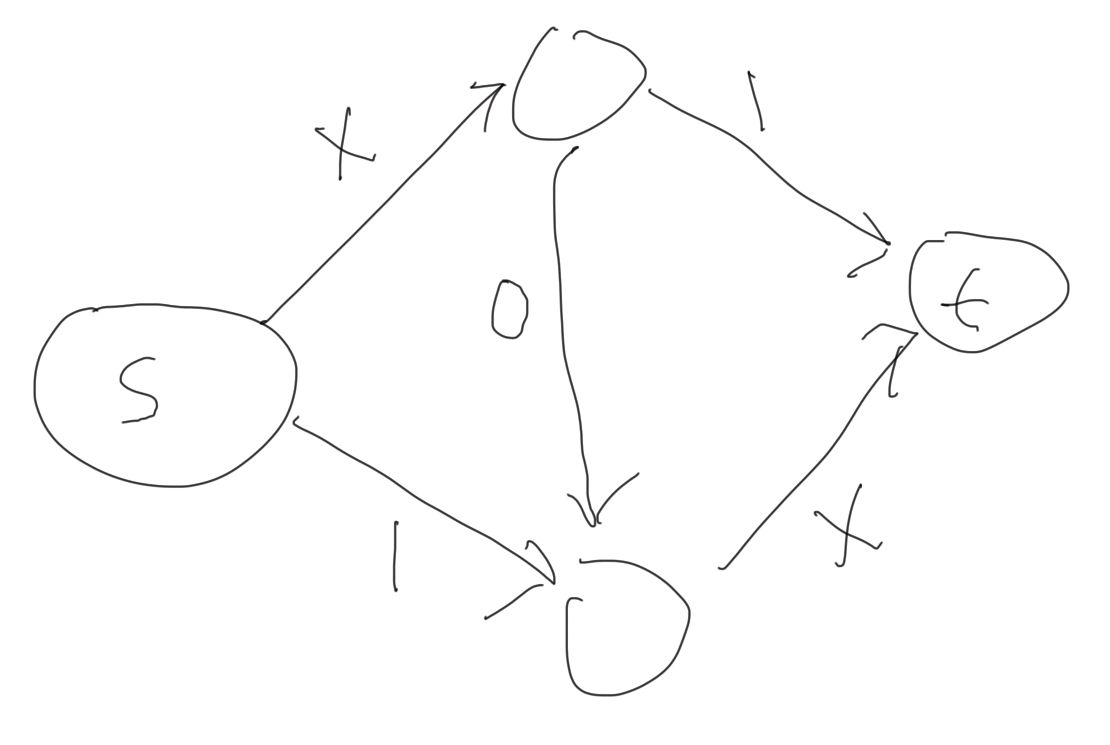
\includegraphics[scale=0.4]{braess}
	\caption{Routing game from s to t. Strategic interaction will make everyone worse off.}
	\label{braess}
\end{figure}
In this game, each player chooses which edges to take from the source $s$ to reach the terminal $t$ and try to do it in the least time, total weight of edges taken, as possible. For the edges labeled x, x is equal to the proportion of players who take the route. For example if $50 \%$ of the players take that edge then $x=0.5$. This can be seen as analogous to traffic when driving a car, the more people take a road, the slower the traffic goes and the longer it takes to get somewhere. Knowing this, each player must choose which path to take to get to their destination as quickly as possible. As you can quickly verify, the best solution for society, minimizing the total driving time for all, is when half of the drivers take the top route, and half of the drivers take the bottom route taking in total 1.5 for each driver. 

\begin{figure}[h!]
	\centering
	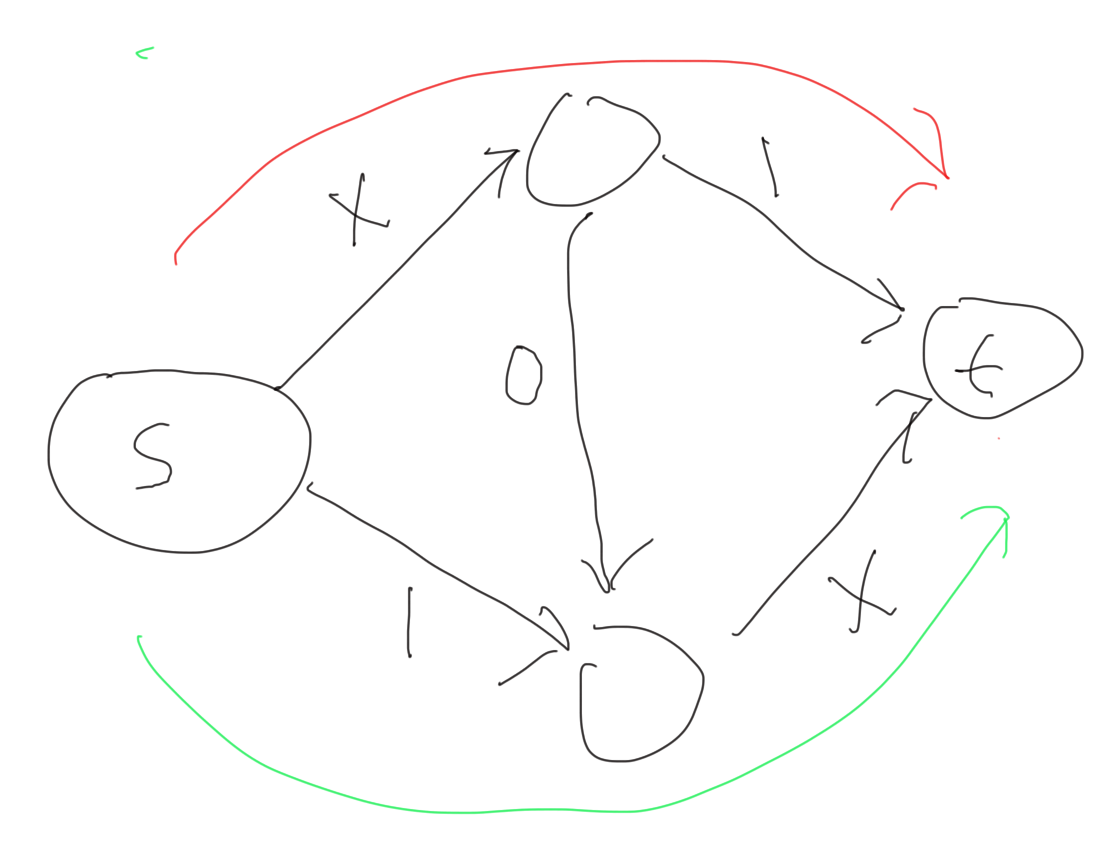
\includegraphics[scale=0.4]{braess_2}
	\caption{Socially optimal route: half taking top, half taking bottom}
	\label{braess2}
\end{figure}

However, this is not an equilibrium. The drivers taking the top route have incentive to instead take the middle edge to try and lower their total time traveled. In fact, the Nash equillibrium will end up with all of the drivers taking the top x, going through the middle, and then the bottom x. Only then will no players have reason to deviate. This however, produces a worse outcome for all players. 

\begin{figure}[h!]
	\centering
	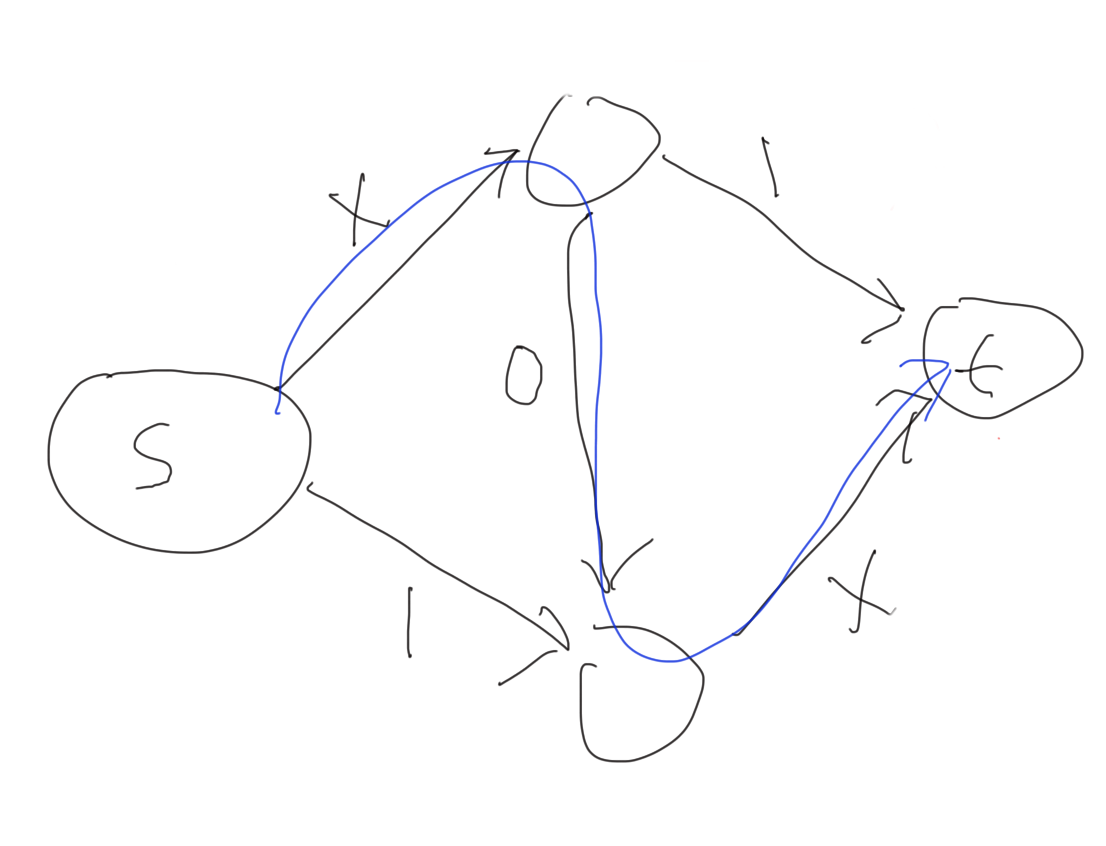
\includegraphics[scale=0.4]{braess_3}
	\caption{Route under strategic interaction}
	\label{braess3}
\end{figure}

Now, it take time 2 for each player to reach the terminal. Thus, under strategic interaction we see that the equilibrium is sub-optimal for society, and in this case all players as well. In this case, the price of anarchy can be computed as $$POA = 2/3$$ (cite Roughgarden lectures)

This framework of the price of anarchy is now being applied to understand auctions by researchers in the algorithmic game theory field. Where for selfish routing games, the price of anarchy has been shown to have a tight bound of 1.5, the question for single price auctions only has approximate upper and lower bounds set on it, and is not known at all for double auctions. Before exploring this further, we should set up the mathematical framework of auctions that is necessary to compute such bounds. An \textbf{auction} is a market mechanism, operating under specific rules that determines to whom one or more items will be awarded and at what price. For a bidder in an auction, the \textbf{value} $v_i$ is the maximum price that bidder $i$ is willing to pay for an item. This is sometimes called a $private valuation$ as this value is generally unknown by the other participants in the auction. The \textbf{bid}, $b_i$, is the off that bidder $i$ submits for for an item. \textbf{Sincere bidding} is when $v_i = b_i$, \textbf{underbidding} is when $v_i > b_i$, and \textbf{overbidding} is when $v_i < b_i$. The highest bid made by any bidder is denoted $b^*$, and is the winning bid (if multiple bids equal the winning bid, then some tie-breaking rule must be used). The \textbf{selling price}, $p^*$ is the final price that the bidder actually pays for the item (which depending on the auction type need not equal $b^*$). Under the \textbf{first-price} rule, the bid submitted by the winner is equal to the selling price. Before the auction begins, each bidder know their personal or private value for the item. An auction consists of a set of bidders, $I = (1,2, ...,N)$ and a seller. After the auction, the bidder $i$ wins the item if their bid is higher than the bid placed by any other bidder $k$ $b_i > max_{k \neq b_k}$. In a single unit auction, the \textbf{income of the bidder} $i$ is equal to their value of the item: $$ \Gamma_i^* = v_i$$ and the \textbf{surplus of the bidder} $i$ is equal to the difference between income and cost $$ \Pi_i^* = \Gamma_i^* - p^*$$. If a bid placed by a bidder is less than the winning bid, they do not win anything and their income and surplus are both zero. The \textbf{sellers revenue} in a single unit auction is equal to the price paid by the winning bidder $$ R^* = p^*.$$ 

Pricing rules in an auction. \textbf{First-Price}: the winning bidder pays the amount of their bid, which is the highest bid of the auction: $p^* = b^*$. Also called \textbf{pay-what-you-bid} (PWYB). \textbf{Second-price}: the winning bidder pays an amount that is equal to the second highest bid for the awarded item. First price auctions will make people tend to bid lower than their private valuation since if they bid that value their profit is zero. Under this rule the item could be awarded to someone who value the item less. Second price auctions encourages bidder to bid their true values (as they will gain positive profits if they win no matter the second highest bid). This encourages an efficient allocation of items (CITE MOSHAN, bibtex error). For the moment we will confine ourselves to first price auctions as this is where most of the strong results in POA analysis of auctions currently are. 

Syrgkanis and Tardos proved in 2013 that the price of anarchy in first price, single item auctions is at least $1 - \frac{1}{e} \approx 0.63$. The exact upper bound on the price of anarchy for single payer, first price auctions remains unknown in the general case. 

This answers the question for what is the price of anarchy at equilibrium, but these results do not pay attention to how the players arrive at there. In real world applications, we expect that players might play repeatedly in the same auction and learn as they play rather than come in with pre-computed strategies. This is especially true for when computing the equilibrium is computationally hard and the stakes of each individual auction is small. Given these observations, it is natural to ask questions about how the efficiency results carry over to adaptive game environments. The model for learning agents that is commonly used in the field is \textbf{no regret learning}. An algorithm for a player satisfies the no-regret condition if, in the limit as the number of times the game is played goes to infinity, the average reward of the algorithm is at least as good as the average reward for the best fixed action in hindsight (assuming the sequence of actions for the other players remains unchanged). If each player  incorporates this kind of learning algorithm, then it has been shown that these can converge to a larger class of equilibrium called correlated equilibrium where each player conditions their response on the expected action of the other player. Now, we can use the following theorem: If an auction is $(\lambda, \mu)$-smooth, then for every valuation profile $\textbf{v}$, every vanishing regret sequence has expected welfare at least $\frac{\lambda}{\mu} \cdot OPT(\textbf{v})$ as $T \rightarrow \infty$. Because we know that a first price single payer auction is a smooth..... \cite{Roughgarden2017} (need to find source finishing jump from POA to no regret learning and giving bounds for single item, first bidder auctions)

With all of this set up, we now state our goal: to simulate no-regret learning algorithms for agents in a first price, single payer auction to see how well the price of anarchy holds. We also want to compare this with other learning algorithms that aren't no regret to see if this framework of using these algorithms is appropriate for making generalizations about equilibrium under learning.

	
\section{Simulated Agents and Simulated Economies}
The use of computers in economics goes back all of the way to general purpose computers being invented in the 1940's. Wassily Leontif used a computer to invert a 39 x 39 matrix to help solve his input output model. Since then, computers use in economics has exploded. With computers economists are able to solve bigger matrices, do Monte-Carlo simulations, create multinomial probit models, and use full information maximum likelihood estimation \cite{Backhouse2016}. While one branch of computational economics is focused on creating stronger and stronger calculators to facilitate empirical research, another branch has focused on creating simulated economies that allow economists to construct a blended version of theory and research within a computer program. Within these simulated economies, theories can be coded into the simulation which when run can allow the researcher to conduct experiments that might not be practical (or ethical) to conduct in the real world. 

One kind of a simulation that can be run is what is an agent-based model (ABM), a simulated system of autonomous decision makers called agents. These models are able to generate complex behavior even if only simple assumptions are made about the behavior of the coded agents. That is, these agents interacting with each other in complex ways are able to produce emergent phenomena in the macro structure of the system that are interesting

For example, in the 1970's Thomas Schilling created a computer simulation to try and understand how and why self segregated neighborhoods formed. Thus, he coded a virtual environment where agents were given preferences to not be a minority where they ended up and move otherwise. From this,  

 
\chapter{Literature Review}
	This "chapter" is my attempt to get words on a page in the process of writing the literature review. It is also an attempt to structure my thought process on what I have read and what questions I want to answer. In general, the proceeding sections would like to answer the following questions:
	
	\begin{itemize}
		\item Why Multi-Agent Simulations?
		\item How do the agents model people, what are the assumptions?
		\item How does learning affect these simulations?
		\item Does the non-stationarity of multi-agent systems make learning techniques invalid as models of human behavior?
	\end{itemize}
	
	Because this is a cursory document it will move back and forth between detailed notes on a single paper and a more structured literature review where I feel stronger on the material.
	
\section{Why use Agent Based Modeling?}
	Tries to answer :
	\begin{itemize}
		\item What questions do Agent Based Models (ABM) try to answer?
		\item What are their strengths?
		\item What are their shortcomings?
		\item Examples and results?
	\end{itemize}

\subsection{The Logic of Agent Based Simulations}

From "Agent-based modeling: Methods and techniques for simulating human systems" \cite{Bonabeau2002}: \\

Agent-based modeling (ABM) is a technique that models a system as a computer simulation of autonomous decision making entities that we call agents. The agents behavior and decision making process should in some way represent the behavior of the system they are supposed to model. Models are able to produce complex behavior from even relatively simple assumptions about agents that may be insightful for understanding the system they are trying to simulate. "Sophisticated ABM sometimes incorporates neural networks, evolutionary algorithms, or other learning techniques to allow realistic learning and adaptation." The main idea of ABM's is "describing a system from the prospective of its constituent units." 

"The benefits of ABM over other modeling techniques can be captured in three statements: (i)  ABM captures emergent phenomena; (ii) ABM provides a natural description of a system; and (iii) ABM is flexible." The main benefit from this list being that ABM captures emergent phenomena that result from the interaction of individual agents. Example given is Traffic Jam that is result of car agents, but the traffic jam moves in the opposite direction of the cars and the traffic jam is itself an emergent behavior from the Car agents. One reason to use and ABM model is if there may be emergent phenomena; " when (i) Individual behavior is nonlinear and can be characterized by thresholds, if-then rules, or nonlinear coupling. (ii) Individual behavior exhibits memory, path dependence, and hysteresis, non-markovian behavior, or temporal correlations including learning and adaptation. (iii) Agent interactions are heterogeneous and can generate network effects. (iv) Averages will not work. Aggergate DEQ's tent to smooth out fluctuations, not ABM, which is important because under certain conditions, fluctuations can be amplified."

ABM is natural for explaining a system of behavioral entities such as traffic jams, stock markets, voters, or the inter-workings of an organization. Modeling Markets: Markets, and stock markets specifically have their resulting dynamics come from the interaction of many agents. This can be understood using ABM. NASDAQ used a an ABM to make decision about mechanism changes where there are many agents who learn via reinforcement learning and neural networks with the goal not being to emulate human behavior, but all possible behavior in regards to the change in mechanism. Found that decreasing tick-size actually increased ask-bid spread and made price discovery harder for agents. Another use is modeling auctions. EBAY lets people build agents to automate the bidding process. \textbf{important to thesis below:} "ultimately, transactions among economic software agents will constitute an essential and perhaps even dominant portion of the world economy." People at IBM have been exploring impact of shopbots on market dynamics with simulated shopbot economies of buyers and sellers. Economists have studied phenomena such as price dispersion by using ABM models where the goal is to design economic software agents. "In particular, they have been examining agent economies in which (i)search costs are nonlinear; (ii) some portion of the buyer population makes no use of search mechanisms; and (iii) shopbots are economically motivated strategically pricing their services so as to maximize their own profits." These stratagies of ABM techniques can also be applied to studying many agents playing an economic game. Author calls this "Game Theory without the theory." and says "Game theory is a great framework, but game theorists suffer from self-imposed constrains: being able to prove their theorems puts severe limitations to what is possible" in particular he argues it is impossible to model realistic games within their framework.

The author describes the following issues with ABM. Like all models (in social sciences especially) the model must serve a purpose and cannot be a general-purpose model. \textbf{important:} 
"Another issue has to do with the very nature of the systems one is modeling with ABM in social sciences: they most often involve human agents, with potentially irrational behavior, subjective choices, and complex psychology--in other words, soft factors, difficult to quantify, calibrate, and sometimes justify." Should only use ABM to justify qualitative results (not quantitative) due to the varying degrees of accuracy input into the simulation. 
\cite{Bonabeau2002} \\

\textbf{How this applies to Thesis:} This goes in depth on the "why" of Agent based modeling, specifically justifying it for bottom up modeling in the cases where that may be the best way to model something in the social sciences. The really interesting parts to me was about markets which highlights more or less exactly what I want to do, looking at markets composed of heterogeneous agents that learn via methods in AI. Some of these models are not even trying to emulate human behavior but just study the dynamics of competitive computer agents in a market setting (or how to build the best agents). The real issue I seem to be focusing in on is, what results can we get from such AI agent models when we know that different learning algorithms behave differently within the context of a non-stationary learning environment. As noted in my notes from a different section, when multiple agents are interacting and learning together they inherently create a non-stationary environment (constantly changing). This constant changing means that only under very specific circumstances and with certain algorithms can it be proved the agents will converge to an (optimal) equilibrium. Can a neural net be said to approximate a humans learning? Probably not, but many simulations use it anyway. Does changing the composition of agents of each learning algorithm change the resulting dynamic in a meaningful way? If so, like I suspect, what can one even learn from such a simulation that generalizes at all to markets of agents artificial or otherwise?  \\  

\textbf{Artificial Adaptive Agents in Economic Theory}, by John H. Holland and John H. Miller.\\

Recent (as of 1991) advances in machine learning offer the possibility of creating artificial adaptive agents (AAA) that can be tested in a wide variety of environments. Creates a complex adaptive system. Subjects that economists study can be classified as complex adaptive systems with networks of interacting agents and dynamic aggregate behavior. Agents in this system are adaptive if they are given some performance measure such as a utility function that they try to maximize over time. AAA models don't require that agents perform technically demanding computations and derivations to optimize their behavior such as classical models imply. 

II Current techniques. AAA can be created using algorithms such as classifier systems, genetic algorithms, neural networks, and reinforcement learning. Wondering how much to outcomes of a system are tied to the learning algorithms used confronts the rationality postulates. "Usually there is only one way to be fully rational, but there are many ways to be less rational." When building theory off of AAA, want robust behavior across algorithm choice. \cite{Holland1991} \\

\textbf{Agent-Based Computational Economics: Growing Economies from the Bottom Up}, by Leigh Tesfastsion 2002
Market economies are complex adaptive systems consisting of a large number of adaptive agents. Local interactions between these agents give rise to macro behavior of the markets which then feedback into the nature of the local interactions. Agent based models give a way to deal with the dual feedback mechanisms between micro and macro economics. Economists have used ABMs to model complex emergent phenomenons such as inductive learning, imperfect competition, endogenous trade network formation, and co-evolution of individual behaviors and economic institutions. Author calls this agent-based computational economics (ACE) (everyone seems to have a different work/ acronym for these). Can think of these models as laboratories to study economies under controlled experimentation. One aspect they study is emergent behaviors and structures in the economy such as they have formed in real life, without top down planning. Another aspect studied with these is mechanism design, what are the effects of certain rules or regulations on the emergent behavior (think of the NASDAQ example in Bonabeau). While we think of these models being purely representative, the advent of the internet and shopbots is blurring these lines as 'real' economies are developing around artificial agents. ACE researches have used many algorithms to represent the learning process of computational agents. Earliest example was genetic algorithms, but now there is also Q-learning, classifier systems. These learning algorithms were initially developed by computer scientists for optimal performance. This is appropriate  for automated economic processes, but might not be for other social simulations. It might even be appropriate for the agents to jointly learn (shared learning / strategy formulation) to improve market conditions. To model humans and real-world economies, the learning algorithm will actually need to incorporate salient characteristics of actual human making. Might have neighborhoods of agents independently co-evolve their strategies. Aware of this, researchers are doing more systematic evaluations of each learning algorithm, and for example Dawid (citation needed) showed that in dynamic multi-agent economies learning via genetic algorithms, the precise parameter configuration can have a large impact on the long run behavior of the economy. The learning study by Rust et al. showed that of thirty computational trading algorithms submitted to a double-auction tournament at the Santa Fe Institute, the winner was a very simple sniping algorithm that would bid at the last minute beating out algorithms that were at the cutting edge of AI. Gode and Sunder (citation needed) did research into continuous double-actions with computational agents found that the efficacy of this market type were derived largely from its structure and not from the learning of the agents (Good Mechanism Design!). Market efficiency levels close to 100 percent were obtained with agents who submitted bids and asks at random. An open question, is how to model the minds of computational agents. Should they only be viewed as logic machines or as controllers for embodied activity? For automated markets, there is no reason that the agents created have to mimic humans, but for modeling real markets, it is crucial to model humans for it to have predictive power. Observed evidence suggests no algorithm performs best in all circumstances, and no algorithm best replicates human behavior. \cite{Tesfatsion2002} \\

\textbf{Agent-Based Computational Economics: A Constructive Approach To Economic Theory} by Leigh Tesfatsion. Published 2005.

This paper goes through an extended example of an agent based simulation of a Walrasian Auctioneer market to show the benefits and drawbacks of the agent based approach. Not finished reading yet, quite long.
\cite{Tesfatsion2005} \\

\textbf{The Complexity of Exchange} by Robert Axtell
Computational complexity of two classes of market mechanisms are compared: the Walrasian market where prices are determined by a central auctioneer and decentralized markets with concurrent exchange between coalitions of agents. An important aspect of agent based models of markets is the price formation process. Through interaction, the prices \textit{emerge} whether through a market maker, or not. Talks about how agent based models don't really try to model equilibrium in the economy, but complexity. Have ecologies of strategies among agents that when tipped in one direction rapidly evolve to a new quasi-equilibrium. 

The complexity of Walrasian Exchange is in NP (Nondeterministic Polynomial time), and is computationally infeasible to be a mechanism for an actual market. (This result is cited)

Complexity of k-lateral exchange equillibria is in P (polynomial time) This result is proved and is the bulk of the paper. Shows that distributed interaction models are easier to compute and represent a better way of being a mechanism for determining prices.
\cite{Axtell2005}\\




\subsection{Game Theory and Computation}
\textbf{Computer Science and Game Theory} by Yoav Shoham (same author as Multi Agent Systems book) Game theory, while initially developed within the discipline of economics has within the beginning part of the 20th century become more and more relevant to computer science. It is integral to artificial intelligence, e-commerce, networking, and other areas of computer science (including cryptography, where Adam Groce uses it). The internet is the main reason that it has become so central as it deals with multiple agents interacting, each with their own information and interests. It is interesting to note that both game theory and computer science grew up at the same time and in the same place in particular with John Von Neumann at Princeton in the 1950s. The area started with exploring the algorithmic complexity of playing and solving games, but also dealt with multi-person operations research and bounded rationality. In modern research, the area of multi-agent learning has received much attention and is called interactive learning in the game theory literature. This is important particularly in the field of AI which is trying to move from learning in a single agent context to learning in a multi-agent environment. When multiple agents learn concurrently, one cannot distinguish between leaning and teaching. In this environment, the 'optimal learning' is no longer well defined. Most game theorists assume agents with an infinite ability to reason. 'Bounded Rationality' however, is an area of research that involves games played by automata. In this context, the author questions if the idea of equilibrium as central in game theory needs to be reconsidered in light of competitions involving agents in markets that performed better when not considering this concept. Most of the effort that goes into making a good, competitive AI goes into thinking about making a good heuristic function, and searching and planning; not reasoning about the opponents behavior. \cite{Shoham2008a}


\subsection{Example: Schelling's Segregation Model}

Schelling's Segregation model is an example of a ABM designed in 1969 by Thomas C. Shelling to try and explain racial segregation. Example of how agent preferences can lead to interesting aggregate structure. This model is presented in the lecture notes of Thomas Sargent and I recreated the model in python. The model is as follows: \\

There are two kinds of agents, orange and green of which there are 250 of each type living in on a unit square. The agents each have a location, a point on the square, $(x,y)$, where $0 < x,y,<1$. The agents are \textit{happy} if half of its neighbors, the ten closest agents in euclidean distance, are of the same type. If the agent is not \textit{happy} then the agent is said to be \textit{unhappy}. Initially, the agents are randomly assigned a point on the unit square i.e. each is initially assigned a point drawn from a bi-variate uniform distribution $ S = (0,1)^2$. Cycling though each agent, each agent is given a choice to stay or to move. If the agent is happy, then they stay otherwise they move according to the following procedure:

\begin{adjustwidth}{1cm}{}
	\textbf{1.} Draw a random location in $S$ \\
	\textbf{2.} If happy at new location, move there\\
	\textbf{3.} Else, go to step 1
\end{adjustwidth}

Continue this cycle, moving through the agents until everyone is happy and does not wish to move.\\

The results are shown in the following figures: 

\begin{figure}[h!]
	\centering
	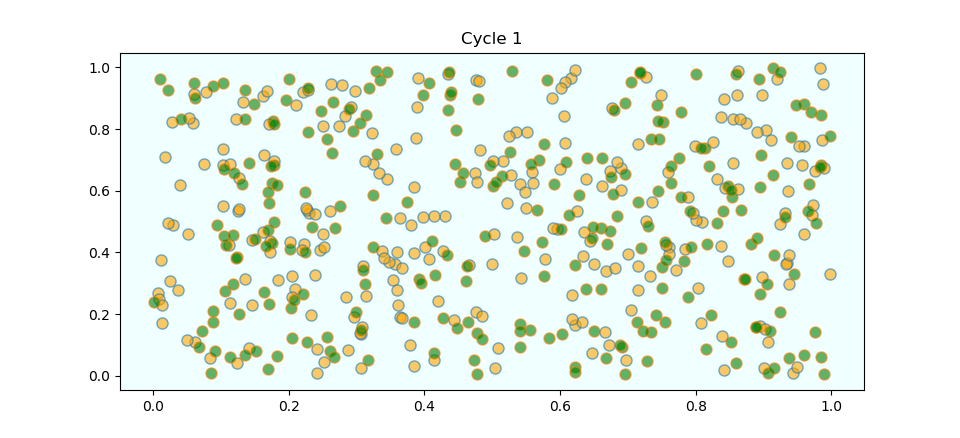
\includegraphics[scale=0.5]{segregation_1}
	\caption{Schelling's Segregation Model: Cycle 1}
	\label{SSM1}
\end{figure}

\begin{figure}[h!]
	\centering
	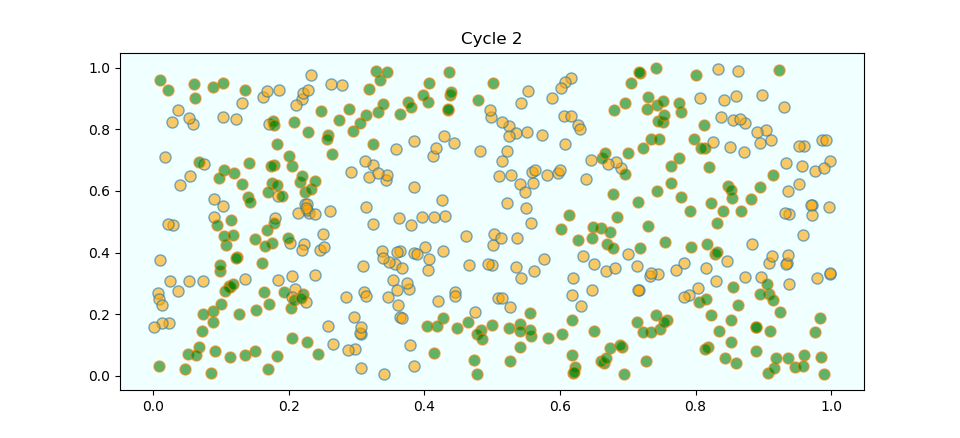
\includegraphics[scale=0.5]{segregation_2}
	\caption{Schelling's Segregation Model: Cycle 2}
	\label{SSM2}
\end{figure}
\begin{figure}[h!]
	\centering
	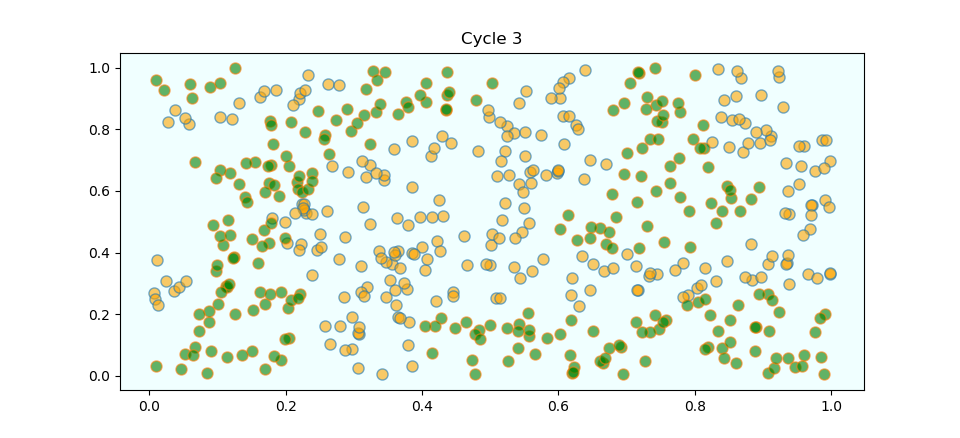
\includegraphics[scale=0.5]{segregation_3}
	\caption{Schelling's Segregation Model: Cycle 3}
	\label{SSM3}
\end{figure}
\begin{figure}[h!]
	\centering
	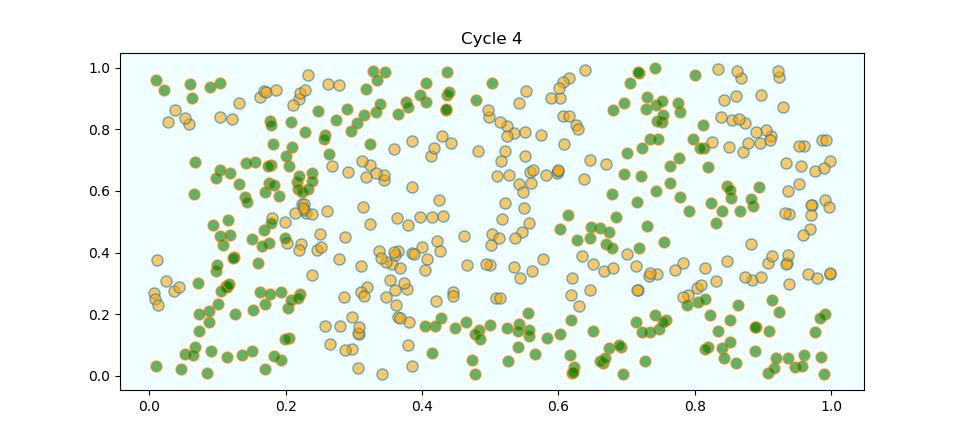
\includegraphics[scale=0.5]{segregation_4}
	\caption{Schelling's Segregation Model: Cycle 4}
	\label{SSM4}
\end{figure}
\begin{figure}[h!]
	\centering
	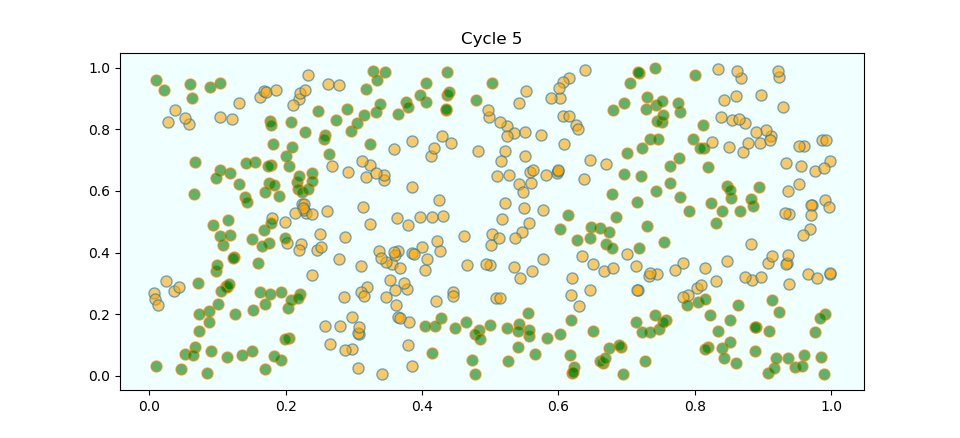
\includegraphics[scale=0.5]{segregation_5}
	\caption{Schelling's Segregation Model: Cycle 5}
	\label{SSM5}
\end{figure}

As can be seen, in cycle 1 (Figure \ref{SSM1}), the agents are well distributed among each other, but as they move in cycles 2-5, they become progressively more segregated. After 5 cycles all agents are happy and the simulation terminates. This example highlights the benefits of using an ABM. With very few assumptions about the agents preferences (wanting half or more of their neighbors to be the same type as them), we can see the resulting emergent behavior of segregated neighborhoods in the system as a whole.


\chapter{Auctions and Markets}
This chapter is about auctions, and artificial simulations in auctions. It will specifically cover what I am reading with reference to the double auction simulation I hope to make. This is separated from the literature review for organizational purposes as I collect my notes, but will be moved there in the future.

\subsection{Basic Notation and Ideas}

From "Understanding Auctions" by Asuncion Mochon and Yago Saez. (TODO: Add citation manually)\\
An \textbf{auction} is a market mechanism, operating under specific rules, that determines to whom one or more items will be awarded and at what price. They are important to environments in which it is difficult to set a market price. For a bidder in an auction, the \textbf{value}, $v_i$ is the maximum price that bidder $i$ is willing to pay for an item. The \textbf{bid}, $b_i$ is the offer that bidder $i$ submits for an item. \textbf{Sincere bidding} is when $v_i = b_i$, \textbf{underbidding} is when $v_i > b_i$, and \textbf{overbidding} is when $v_i < b_i$. The highest bid made by any bidder is denoted $b^*$, and is the winning bid (if multiple bids equal the winning bid, then some tie-breaking rule must be used). The \textbf{selling price}, $p^*$ is the final price that the bidder actually pays for the item (which depending on the auction type need not equal $b^*$). Under the \textbf{first-price} rule, the bid submitted by the winner is equal to the selling price. Before the auction begins, each bidder know their personal or private value for the item. The term \textbf{winner's curse} refers to the idea that the bidder who wins may have paid to much for the item in the sense that no one else was willing to pay near that much for the item. That is, in a first price auction the winner paid extra the difference between their bid and the second highest bid. In some experimental work by Thaler, people tend to respond to the risk of overpaying by decreasing bids with respect to their values. 

An auction consists of a set of bidders, $I = (1,2, ...,N)$ and a seller. After the auction, the bidder $i$ wins the item if their bid is higher than the bid placed by any other bidder $k$ $b_i > max_{k \neq b_k}$. In a single unit auction, the \textbf{income of the bidder} $i$ is equal to their value of the item: $$ \Gamma_i^* = v_i$$ and the \textbf{surplus of the bidder} $i$ is equal to the difference between income and cost $$ \Pi_i^* = \Gamma_i^* - p^*$$. If a bid placed by a bidder is less than the winning bid, they do not win anything and their income and surplus are both zero. The \textbf{sellers revenue} in a single unit auction is equal to the price paid by the winning bidder $$ R^* = p^*.$$ 

Pricing rules in an auction. \textbf{First-Price}: the winning bidder pays the amount of their bid, which is the highest bid of the auction: $p^* = b^*$. Also called \textbf{pay-what-you-bid} (PWYB). \textbf{Second-price}: the winning bidder pays an amount that is equal to the second highest bid for the awarded item. First price auctions will make people tend to bid lower than their private valuation since if they bid that value their profit is zero. Under this rule the item could be awarded to someone who value the item less. Second price auctions encourages bidder to bid their true values (as they will gain positive profits if they win no matter the second highest bid). This encourages an efficient allocation of items.

\textbf{Optimal Auctions} are those that maximize the expected revenue for the seller.
\textbf{Efficient Auctions} are those that the items are awarded to the bidders who most value them.
These goals are often conflicting.

\textbf{Double Auctions} The main characteristic of a double auction is that multiple buyers and sellers interact, making it a two sided auction. In a double auction, buyers submit bids for the amount they are willing to pay, and sellers make offers, asks, for the price they are willing to sell. A synchronized continuous double auction is composed of $r$ rounds, which are divided into $s$ periods. In each period, there are a fixed number of $t$ steps which alternate steps in which buy and sell orders are placed. Each step $t$ begins with a bid/ask step in which, simultaneously, the buyers indicate the prices that they are willing to pay per unit, and the sellers indicate the prices at which they are willing to sell. \\
 

Notes for "The Double Auction Market: Institutions, Theories, and Evidence. Edited by Daniel Friedman and John Rut\\

Ch. 1 "The Double Auction Market Institution: A survey" by Daniel Friedman \\

The continuous double auction allows traders to make offers to buy or sell and accept other traders' offers at any moment during a trading period. For past 100 years NY, London, and Chicago exchanges all operate under some form of double auction rules. Laboratory experiments show that double auctions continuously produce very efficient prices and allocations, more so than theory would suggest.\\

Notes from "Bidding Strategies in Agent-Based Continuous Double Auctions" by Huiye Ma and Ho-fung Leung

In continuous double auctions (CDA), buyers submit increasingly higher bids and sellers submit increasingly lower asks at any moment during a trading period and transactions occur when the highest bid is at least as high as the lowest ask. Auctions in general consist of two components: protocols and strategies. The former is the rules each agent must abide by in the auction and the latter is the way that the agent tries to achieve their means within that protocol.\\

\textbf{Basic CDA Mechanisms}\\
Is a marketplace where there are agents selling goods (sellers) and agents buying goods (buyers). The sellers and buyers trade homogeneous goods. The current lowest ask is called the outstanding ask, $oa$. The current highest bid is called the outstanding bid, $ob$. A valid bid is a bid higher than the current $ob$ and similarly a valid ask is any ask lower than current $oa$. Any invalid bid/ask is ignored by the market. Each buyer and seller has an acceptable price range $[]P_{ll}, P_{ul}$ for a CDA. $P_{ll}$ is the lowest acceptable price and $P_{ul}$ is the highest acceptable price. This range is formed on experience. Each buyer and seller has a reservation price that can be thought of as their valuation of the good. Buying a good for more then that or selling for less then that would cause the buyer/seller to lose profit. When the $ob$ is higher than or equal to the $oa$, the agents who submitted those bids and asks will make a transaction. When there is a transaction or a specified time has passed, the round is terminated. A new round can then begin. Only one unit of good is transacted per round. The demand is the total number of goods that buyers want to buy and the supply is the total number of goods that sellers want to sell.

At this point the author lists an algorithm (in pseudo code) for running the market. The author then goes on to give basic trading strategies and their pseudo code for zero intelligence traders and the like.\\

references to check:\\
A Bannall: Autonomous adaptive agents for single seller sealed bid auctions.\\
R. Das: Agent-human interactions in the continuous double auction.\\
S. Gjerstad: Price formation in double auctions\\
D.K. Gode: Allocative Efficiency of markets with zero-intelligence traders.\\
M. He A fuzzy-logic based bidding strategy for autonomous agents in continuous double auctions.\\
C. Preist: Economic Dynamics of agents in multiple auctions.\\
C. Preist: Adaptive agents in a persistent shout double auction.\\
V. Smith: an experimental study of competitive market behavior.\\
M.P. Wellman: Empirical game-theoretic analysis of the tac market games.\\
M.P. Wellman: Designing the market game for a trading agent competition.\\

Simple Agents, Intelligent Markets by Karim Jamal\\
Economics usually focuses in on equilibrium achieved by rational agents who optimize their utility functions. Exploration to th extent at which equilibrium arises from the characteristics of the environment have been limited.  Normally, representative agents in models have sophisticated computational abilities who solve for equilibrium. Plott and Sunder have shown that markets with uncertainty and asymmetrically distributed information disseminate information and converge near rational expectation equilibrium when populated with profit-motivated human traders. This paper shows that the same result can be achieved with minimally intelligent traders in a computer simulation. 
\cite{Jamal2017}



	
\chapter{Agent Systems}
   	This chapter lays out the background material of multi-agent systems--what they are, how they work, and why economists might be interested in them--that drives the rest of the thesis. 
	
\section{Agents}
An \textbf{agent} is something that acts. This comes from the Latin word agere, to do. In general, anything might be considered an agent so long as it can perceive the environment and act upon it. A \textbf{rational agents} is something that acts to achieve the best outcome or with uncertainty, the best expected outcome in a given situation. For example we are agents, we have the ability to take an action and effect the world. We even might be considered rational since we are generally trying to navigate the world around us so as to try and lead to our preferred outcome. People are not the only agents, animals and machines are also agents capable of acting on the world around them. 

\subsection{In Economics}
In economics many of the models are constructed with utility maximizing agents in line with Decision Theory and Rational Choice Theory. Because economics seeks to understand the outcomes of peoples interactions, and perhaps how these outcomes could be improved, if people can be modeled as utility maximizers, it is then possible to analytically solve for this solution and see what the results are. 

The primary purpose of constructing agents in economics is to see how their interactions play out in an economic setting that can not be solved analytically.  
 
\subsection{In Artificial Intelligence}\label{commands}
In artificial intelligence, the primary purpose of understanding agents is to try and create the most effective artificial agents possible. This discipline cares deeply about how good the agents they are able to make are able to solve problems, either general or specific. To do this, they use much of the theory of agents with a deep emphasis on how a constructed agent can be taught or learn from its environment to achieve its goals.


	
\section{Formal Model of Agents}
This section lays out a more formal definition of agents, specifically geared towards constructed or artificial agents such as we will be constructing. An \textbf{agent} is anything that can be viewed as perceiving its environment through sensors and acting upon its environment through actuators. A \textbf{precept} is a perceptual input to an agent, and a \textbf{precept sequence} is the complete history of everything the agent has ever perceived. The agent then has an \textbf{agent function} that maps these precepts to an action. In the case of an artificial agent this is done with an \textbf{agent program} that is the physical implementation of the agent function. In the case of an agent simulated on a computer, this will be the computer code that decides what action to take. The agents actions will then cause the environment to go through a series of states and the agent will measure the outcome with some \textbf{performance measure}.

%\begin{figure}[h!]
%	% the options are h = here, t = top, b = bottom, p = page of figures.
%	% you can add an exclamation mark to make it try harder, and multiple
%	% options if you have an order of preference, e.g.
%	% \begin{figure}[h!tbp]
%	
%	\centering
%	% DO NOT ADD A FILENAME EXTENSION TO THE GRAPHIC FILE
%	\includegraphics[scale=0.05, angle=90]{utilityAgent}
%	\caption{Utility Based Agent}
%	\label{utility-agent-STOLEN}
%\end{figure}

For our purposes we focus on what are called \textbf{utility based agents}, where the agent has a utility function as an internalized performance measure and is able to numerically assign values of "goodness" to the outcome from the agents perspective. A rational agent will always try to maximize average expected utility over its lifetime as explained by decision theory.

\subsection{Task Environment}
The environment that an agent exists in and their relationship to it is critical for understanding the system as a whole. For example the environment can fully observable with the agent's sensors able to see the entire environment, or only partially observable to the agent. There can also be multiple agents within the system, each trying to maximize their own performance measure. This is called a \textbf{multi-agent system} and it will be a key aspect of all of the simulations we construct. It is important to note that the agents in the multi-agent system share no internal state and must communicate (if they so wish to do so) through the environment. The environment can also be deterministic or stochastic, either depending entirely upon its current state and the agents actions or contains randomness.
	
\subsection{Agents Who Learn}

Learning is a critical part of being a rational agent. We expect that as agents interact with their environment, they should be able to adapt and change in order to continue to maximize their utility. The general model of an artificial agent who learns is as follows. 


%\begin{figure}[h]
%	\centering
%	\includegraphics[scale=0.05]{learningAgent}
%	\caption{Model of Agent that Learns}
%	\label{learning-agent-STOLEN}
%\end{figure}

First, the agent reprieves its environment and sends that information to the performance function that determines what it will do. There is now a critic that gives feedback for how the agent is doing based on aprori information and the observed state that sends feedback to a learning element that can change the behavior of the performance element. Based on what the learning element is trying improve, there is also a problem generator that suggests actions to the performance element so that different actions can be tested and evaluated. \cite{Russel2010}
\chapter{Reinforcement Learning}	

Reinforcement learning has become a popular way of teaching agents how to play games and interact with each other in Machine Learning (ML). Because the dynamics and behavior of a final simulation are determined by the learning algorithm used for its composing agents, we spend some time developing the ideas of reinforcement learning in both a single agent and multi-agent setting. 
\section{Single Agent Learning}
	Reinforcement learning is the area of machine learning where agents learn through repeated interactions with their dynamic environment. This section gives a brief overview of learning algorithms used by single agents with a focus on deep reinforcement learning. In general, reiforcment learning formalizes the interaction of agents and environment using a Markov decision process (MDP).\\
	
	\textbf{Definition:} Markov Decision Process \\
	A Markov decision process is 5-tuple $ \langle \mathcal{S, A,} R, T, \gamma \rangle $ where, \\
	\textbf{1.} $\mathcal{S}$ represents a finite set of states \\
	\textbf{2.} $\mathcal{A}$ represents a finite set of actions \\
	\textbf{3.} $T$ is a transition function $T: \mathcal{S} \times \mathcal{A} \times \mathcal{S} \rightarrow [0,1]$ that determines the probability of transitioning from any state $s \in \mathcal{S}$ to any state $s^{'} \in \mathcal{S}$ given any possible action $a \in A$\\
	\textbf{4.} $R$ is the reward function $R: \mathcal{S} \times \mathcal{A} \times \mathcal{S} \rightarrow \mathbb{R}$\\
	\textbf{5.} $\gamma \in [0,1]$ is the discount factor that balances immediate and future rewards
	
	
\subsection{Q-Learning}
Q-Learning is an an algorithm that has been developed for single-agent, fully observable environments with discrete actions. Q learning involves creating a table of expected payoffs for each action $a$ available at a state $s$ denoted $\hat{Q}(s,a)$. Each time the agent transitions from a state $s$ to a state $s^{'}$ taking an action $a$ and recieving payoff $r$, the $Q$ table is updated according to the following assignment:
$$ \hat{Q}(s,a) \leftarrow \hat{Q}(s,a) + \alpha [(r + \gamma max_{a^{1}} \hat{Q}(s^{'}, a^{'})) - \hat{Q}(s,a)] $$

where we pick $\alpha \in [0,1]$ which we call the learning rate.

\subsection{Deep Reinforcement Learning}
Using deep learning in the form of Neural Networks can be helpful for exploring large policy spaces efficiently. It also eliminates the need to hand design features to be optimized for the reinforcement learning process. \cite{Shoham2008} 



\chapter{Tables and Graphics}

\section{Tables}
	The following section contains examples of tables, most of which have been commented out for brevity. (They will show up in the .tex document in red, but not at all in the .pdf). For more help in constructing a table (or anything else in this document), please see the LaTeX pages on the CUS site. 

\begin{table}[htbp] % begins the table floating environment. This enables LaTeX to fit the table where it works best and lets you add a caption.
\caption[Correlation of Inheritance Factors between Parents and Child]{Correlation of Inheritance Factors between Parents and Child} 
% The words in square brackets of the caption command end up in the Table of Tables. The words in curly braces are the caption directly over the table.
\begin{center} 
% makes the table centered
\begin{tabular}{c c c c} 
% the tabular environment is used to make the table itself. The {c c c c} specify that the table will have four columns and they will all be center-aligned. You can make the cell contents left aligned by replacing the Cs with Ls or right aligned by using Rs instead. Add more letters for more columns, and pipes (the vertical line above the backslash) for vertical lines. Another useful type of column is the p{width} column, which forces text to wrap within whatever width you specify e.g. p{1in}. Text will wrap badly in narrow columns though, so beware.
\toprule % a horizontal line, slightly thicker than \hline, depends on the booktabs package
  Factors &  Correlation between Parents \& Child & Inherited \\ % the first row of the table. Separate columns with ampersands and end the line with two backslashes. An environment begun in one cell will not carry over to adjacent rows.
  \midrule % another horizontal line
	Education 				& -0.49 & Yes 	 \\ % another row
	Socio-Economic Status 	& 0.28 	& Slight \\
	Income 					& 0.08 	& No	 \\
	Family Size 			& 0.19 	& Slight \\
	Occupational Prestige 	& 0.21 	& Slight \\
\bottomrule % yet another horizontal line
\end{tabular}
\end{center}
\label{inheritance} % labels are useful when you have more than one table or figure in your document. See our online documentation for more on this.
\end{table}

	\clearpage 
%% \clearpage ends the page, and also dumps out all floats. 
%% Floats are things like tables and figures.

If you want to make a table that is longer than a page, you will want to use the longtable environment. Uncomment the table below to see an example, or see our online documentation.

%% An example of a long table, with headers that repeat on each subsequent page: Results from the summers of 1998 and 1999 work at Reed College done by Grace Brannigan, Robert Holiday and Lien Ngo in 1998 and Kate Brown and Christina Inman in 1999.

	\begin{longtable}{||c|c|c|c||}
	 	\caption[Chromium Hexacarbonyl Data Collected in 1998--1999]{Chromium Hexacarbonyl Data Collected in 1998--1999}\\ \hline
	    	  \multicolumn{4}{||c||}{Chromium Hexacarbonyl} \\\hline
		   State & Laser wavelength & Buffer gas & Ratio of $\frac{\textrm{Intensity
at vapor pressure}}{\textrm{Intensity at 240 Torr}}$ \\ \hline
		  \endfirsthead
		\hline     State & Laser wavelength & Buffer gas & Ratio of
$\frac{\textrm{Intensity at vapor pressure}}{\textrm{Intensity at 240 Torr}}$\\
\hline
		    \endhead

	    $z^{7}P^{\circ}_{4}$ & 266 nm & Argon & 1.5 \\\hline
	    $z^{7}P^{\circ}_{2}$ & 355 nm & Argon & 0.57 \\\hline
	    $y^{7}P^{\circ}_{3}$ & 266 nm & Argon & 1 \\\hline
	    $y^{7}P^{\circ}_{3}$ & 355 nm & Argon & 0.14 \\\hline
	    $y^{7}P^{\circ}_{2}$ & 355 nm & Argon & 0.14 \\\hline
	    $z^{5}P^{\circ}_{3}$ & 266 nm & Argon & 1.2 \\\hline
	    $z^{5}P^{\circ}_{3}$ & 355 nm & Argon & 0.04 \\\hline
	    $z^{5}P^{\circ}_{3}$ & 355 nm & Helium & 0.02 \\\hline
	    $z^{5}P^{\circ}_{2}$ & 355 nm & Argon & 0.07 \\\hline
	    $z^{5}P^{\circ}_{1}$ & 355 nm & Argon & 0.05 \\\hline
	    $y^{5}P^{\circ}_{3}$ & 355 nm & Argon & 0.05, 0.4 \\\hline
	    $y^{5}P^{\circ}_{3}$ & 355 nm & Helium & 0.25 \\\hline
	    $z^{5}F^{\circ}_{4}$ & 266 nm & Argon & 1.4 \\\hline
	    $z^{5}F^{\circ}_{4}$ & 355 nm & Argon & 0.29 \\\hline
	    $z^{5}F^{\circ}_{4}$ & 355 nm & Helium & 1.02 \\\hline
	    $z^{5}D^{\circ}_{4}$ & 355 nm & Argon & 0.3 \\\hline
	    $z^{5}D^{\circ}_{4}$ & 355 nm & Helium & 0.65 \\\hline
	    $y^{5}H^{\circ}_{7}$ & 266 nm & Argon & 0.17 \\\hline
	    $y^{5}H^{\circ}_{7}$ & 355 nm & Argon & 0.13 \\\hline
	    $y^{5}H^{\circ}_{7}$ & 355 nm & Helium & 0.11 \\\hline
	    $a^{5}D_{3}$ & 266 nm & Argon & 0.71 \\\hline
	    $a^{5}D_{2}$ & 266 nm & Argon & 0.77 \\\hline
	    $a^{5}D_{2}$ & 355 nm & Argon & 0.63 \\\hline
	    $a^{3}D_{3}$ & 355 nm & Argon & 0.05 \\\hline
	    $a^{5}S_{2}$ & 266 nm & Argon & 2 \\\hline
	    $a^{5}S_{2}$ & 355 nm & Argon & 1.5 \\\hline
	    $a^{5}G_{6}$ & 355 nm & Argon & 0.91 \\\hline
	    $a^{3}G_{4}$ & 355 nm & Argon & 0.08 \\\hline
	    $e^{7}D_{5}$ & 355 nm & Helium & 3.5 \\\hline
	    $e^{7}D_{3}$ & 355 nm & Helium & 3 \\\hline
	    $f^{7}D_{5}$ & 355 nm & Helium & 0.25 \\\hline
	    $f^{7}D_{5}$ & 355 nm & Argon & 0.25 \\\hline
	    $f^{7}D_{4}$ & 355 nm & Argon & 0.2 \\\hline
	    $f^{7}D_{4}$ & 355 nm & Helium & 0.3 \\\hline
	    \multicolumn{4}{||c||}{Propyl-ACT} \\\hline
%	    State & Laser wavelength & Buffer gas & Ratio of $\frac{\textrm{Intensity
%at vapor pressure}}{\textrm{Intensity at 240 Torr}}$\\ \hline
	    $z^{7}P^{\circ}_{4}$ & 355 nm & Argon & 1.5 \\\hline
	    $z^{7}P^{\circ}_{3}$ & 355 nm & Argon & 1.5 \\\hline
	    $z^{7}P^{\circ}_{2}$ & 355 nm & Argon & 1.25 \\\hline
	    $z^{7}F^{\circ}_{5}$ & 355 nm & Argon & 2.85 \\\hline
	    $y^{7}P^{\circ}_{4}$ & 355 nm & Argon & 0.07 \\\hline
	    $y^{7}P^{\circ}_{3}$ & 355 nm & Argon & 0.06 \\\hline
	    $z^{5}P^{\circ}_{3}$ & 355 nm & Argon & 0.12 \\\hline
	    $z^{5}P^{\circ}_{2}$ & 355 nm & Argon & 0.13 \\\hline
	    $z^{5}P^{\circ}_{1}$ & 355 nm & Argon & 0.14 \\\hline
	    \multicolumn{4}{||c||}{Methyl-ACT} \\\hline
%	    State & Laser wavelength & Buffer gas & Ratio of $\frac{\textrm{Intensity
% at vapor pressure}}{\textrm{Intensity at 240 Torr}}$\\ \hline
	    $z^{7}P^{\circ}_{4}$ & 355 nm & Argon & 1.6, 2.5 \\\hline
	    $z^{7}P^{\circ}_{4}$ & 355 nm & Helium & 3 \\\hline
	    $z^{7}P^{\circ}_{4}$ & 266 nm & Argon & 1.33 \\\hline
	    $z^{7}P^{\circ}_{3}$ & 355 nm & Argon & 1.5 \\\hline
	    $z^{7}P^{\circ}_{2}$ & 355 nm & Argon & 1.25, 1.3 \\\hline
	    $z^{7}F^{\circ}_{5}$ & 355 nm & Argon & 3 \\\hline
	    $y^{7}P^{\circ}_{4}$ & 355 nm & Argon & 0.07, 0.08 \\\hline
	    $y^{7}P^{\circ}_{4}$ & 355 nm & Helium & 0.2 \\\hline
	    $y^{7}P^{\circ}_{3}$ & 266 nm & Argon & 1.22 \\\hline
	    $y^{7}P^{\circ}_{3}$ & 355 nm & Argon & 0.08 \\\hline
	    $y^{7}P^{\circ}_{2}$ & 355 nm & Argon & 0.1 \\\hline
	    $z^{5}P^{\circ}_{3}$ & 266 nm & Argon & 0.67 \\\hline
	    $z^{5}P^{\circ}_{3}$ & 355 nm & Argon & 0.08, 0.17 \\\hline
	    $z^{5}P^{\circ}_{3}$ & 355 nm & Helium & 0.12 \\\hline
	    $z^{5}P^{\circ}_{2}$ & 355 nm & Argon & 0.13 \\\hline
	    $z^{5}P^{\circ}_{1}$ & 355 nm & Argon & 0.09 \\\hline
	    $y^{5}H^{\circ}_{7}$ & 355 nm & Argon & 0.06, 0.05 \\\hline
	    $a^{5}D_{3}$ & 266 nm & Argon & 2.5 \\\hline
	    $a^{5}D_{2}$ & 266 nm & Argon & 1.9 \\\hline
	    $a^{5}D_{2}$ & 355 nm & Argon & 1.17 \\\hline
	    $a^{5}S_{2}$ & 266 nm & Argon & 2.3 \\\hline
	    $a^{5}S_{2}$ & 355 nm & Argon & 1.11 \\\hline
	    $a^{5}G_{6}$ & 355 nm & Argon & 1.6 \\\hline
	    $e^{7}D_{5}$ & 355 nm & Argon & 1 \\\hline

		\end{longtable}

   
   \section{Figures}
   
	If your thesis has a lot of figures, \LaTeX\ might behave better for you than that other word processor.  One thing that may be annoying is the way it handles ``floats'' like tables and figures. \LaTeX\ will try to find the best place to put your object based on the text around it and until you're really, truly done writing you should just leave it where it lies.   There are some optional arguments to the figure and table environments to specify where you want it to appear; see the comments in the first figure.

	If you need a graphic or tabular material to be part of the text, you can just put it inline. If you need it to appear in the list of figures or tables, it should be placed in the floating environment. 
	
	To get a figure from StatView, JMP, SPSS or other statistics program into a figure, you can print to pdf or save the image as a jpg or png. Precisely how you will do this depends on the program: you may need to copy-paste figures into Photoshop or other graphic program, then save in the appropriate format.
	
	Below we have put a few examples of figures. For more help using graphics and the float environment, see our online documentation.
	
	And this is how you add a figure with a graphic:
	\begin{figure}[h]
	% the options are h = here, t = top, b = bottom, p = page of figures.
	% you can add an exclamation mark to make it try harder, and multiple
	% options if you have an order of preference, e.g.
	% \begin{figure}[h!tbp]
	   
	       \centering
	    % DO NOT ADD A FILENAME EXTENSION TO THE GRAPHIC FILE
	    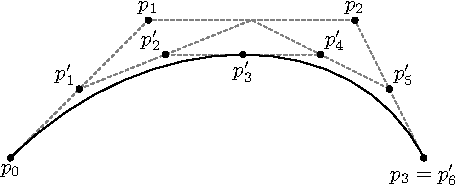
\includegraphics{subdivision}
	     \caption{A Figure}
	 \label{subd}
	\end{figure}

\clearpage %% starts a new page and stops trying to place floats such as tables and figures

\section{More Figure Stuff}
You can also scale and rotate figures.
 	\begin{figure}[h!]
	   
	       \centering
	    % DO NOT ADD A FILENAME EXTENSION TO THE GRAPHIC FILE
	    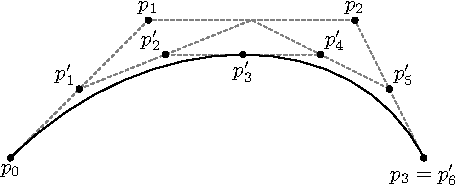
\includegraphics[scale=0.5,angle=180]{subdivision}
	    % if your figure shows up not where you want it, it may just be too big to fit. You can use the scale argument to shrink it, e.g. scale=0.85 is 85 percent of the original size. 
	     \caption{A Smaller Figure, Flipped Upside Down}
	 \label{subd2}
	\end{figure}

\section{Even More Figure Stuff}
With some clever work you can crop a figure, which is handy if (for instance) your EPS or PDF is a little graphic on a whole sheet of paper. The viewport arguments are the lower-left and upper-right coordinates for the area you want to crop.

 	\begin{figure}[h!]
	    	       \centering
	    % DO NOT ADD A FILENAME EXTENSION TO THE GRAPHIC FILE
	   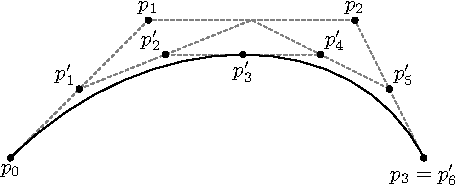
\includegraphics[clip=true, viewport=.0in .0in 1in 1in]{subdivision}
	    \caption{A Cropped Figure}
	 \label{subd3}
	\end{figure}
	
      \subsection{Common Modifications}
      The following figure features the more popular changes thesis students want to their figures. This information is also on the web at \url{web.reed.edu/cis/help/latex/graphics.html}.
    %\renewcommand{\thefigure}{0.\arabic{figure}} 	% Renumbers the figure to the type 0.x
    %\addtocounter{figure}{4} 						% starts the figure numbering at 4
    \begin{figure}[htbp]
    \begin{center}
   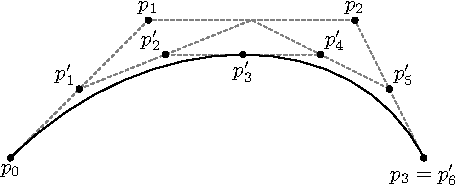
\includegraphics[scale=0.5]{subdivision}
    \caption[Subdivision of arc segments]{\footnotesize{Subdivision of arc segments. You can see that $ p_3 = p_6^\prime$.}} %the special ToC caption is in square brackets. The \footnotesize makes the figure caption smaller
    \label{barplot}
    \end{center}
    \end{figure} 

\chapter*{Conclusion}
         \addcontentsline{toc}{chapter}{Conclusion}
	\chaptermark{Conclusion}
	\markboth{Conclusion}{Conclusion}
	\setcounter{chapter}{4}
	\setcounter{section}{0}
	
Here's a conclusion, demonstrating the use of all that manual incrementing and table of contents adding that has to happen if you use the starred form of the chapter command. The deal is, the chapter command in \LaTeX\ does a lot of things: it increments the chapter counter, it resets the section counter to zero, it puts the name of the chapter into the table of contents and the running headers, and probably some other stuff. 

So, if you remove all that stuff because you don't like it to say ``Chapter 4: Conclusion'', then you have to manually add all the things \LaTeX\ would normally do for you. Maybe someday we'll write a new chapter macro that doesn't add ``Chapter X'' to the beginning of every chapter title.

\section{More info}
And here's some other random info: the first paragraph after a chapter title or section head \emph{shouldn't be} indented, because indents are to tell the reader that you're starting a new paragraph. Since that's obvious after a chapter or section title, proper typesetting doesn't add an indent there. 


%If you feel it necessary to include an appendix, it goes here.
    \appendix
      \chapter{The First Appendix}
      \chapter{The Second Appendix, for Fun}


%This is where endnotes are supposed to go, if you have them.
%I have no idea how endnotes work with LaTeX.

  \backmatter % backmatter makes the index and bibliography appear properly in the t.o.c...

% if you're using bibtex, the next line forces every entry in the bibtex file to be included
% in your bibliography, regardless of whether or not you've cited it in the thesis.
    \nocite{*}

% Rename my bibliography to be called "Works Cited" and not "References" or ``Bibliography''
% \renewcommand{\bibname}{Works Cited}

%    \bibliographystyle{bsts/mla-good} % there are a variety of styles available; 
%  \bibliographystyle{plainnat}
% replace ``plainnat'' with the style of choice. You can refer to files in the bsts or APA 
% subfolder, e.g. 
 \bibliographystyle{APA/apa-good}  % or
 \bibliography{thesis}
 % Comment the above two lines and uncomment the next line to use biblatex-chicago.
 %\printbibliography[heading=bibintoc]

% Finally, an index would go here... but it is also optional.
\end{document}
